\documentclass[12pt,a4paper]{article}
\usepackage[utf8]{inputenc}
\usepackage[spanish]{babel}
\usepackage{graphicx}
\usepackage{float}
\usepackage{geometry}
\usepackage{fancyhdr}
\usepackage{hyperref}
\usepackage{xcolor}
\usepackage{titlesec}
\usepackage{caption}

\geometry{left=2.5cm,right=2.5cm,top=2.5cm,bottom=2.5cm}

\hypersetup{
    colorlinks=true,
    linkcolor=blue,
    urlcolor=blue,
}

\pagestyle{fancy}
\fancyhf{}
\fancyhead[L]{Fotogrametr\'ia --- Sello ESPE}
\fancyfoot[C]{\thepage}

\titleformat{\section}{\Large\bfseries}{\thesection.}{0.5em}{}
\titleformat{\subsection}{\large\bfseries}{\thesubsection.}{0.5em}{}

\begin{document}

% =================== PORTADA ===================
\begin{titlepage}
    \centering
    \vspace*{2cm}
    {\Huge \bfseries Universidad de las Fuerzas Armadas ESPE\par}
    \vspace{1.5cm}
    {\Large Fotogrametr\'ia Aplicada:\\[0.3cm]
    Escaneo 3D del Sello Institucional\par}
    \vspace{2cm}
    {\large \textbf{Asignatura:} Gr\'afica por Computadora\par}
    \vspace{0.5cm}
    {\large \textbf{Estudiante:} Josu\'e Chango\par}
    \vspace{0.5cm}
    {\large \textbf{NRC:} 30720\par}
    \vspace{0.5cm}
    {\large \textbf{Fecha:} \today\par}
    \vfill
\end{titlepage}

% =================== OBJETIVO ===================
\section{Objetivo}

Aplicar el proceso b\'asico de captura y generaci\'on de un modelo 3D mediante fotogrametr\'ia, utilizando la aplicaci\'on Polycam, considerando aspectos como iluminaci\'on, \'angulos de captura, estabilidad y calidad del resultado final.

% =================== SELECCIÓN DEL ELEMENTO ===================
\section{Selecci\'on del Elemento}

Se seleccion\'o el \textbf{sello institucional de la Universidad de las Fuerzas Armadas ESPE}, ubicado en la plazoleta frente a la biblioteca. Se eligi\'o por sus caracter\'isticas geom\'etricas: superficies con relieve, detalles grabados, bordes definidos y un tama\~no que permite capturarlo por completo desde varios \'angulos.

\begin{figure}[H]
    \centering
    \includegraphics[width=0.7\textwidth]{sello_original.jpg}
    \caption{Sello institucional de la ESPE ubicado frente a la biblioteca.}
\end{figure}

% =================== PROCESO DE ESCANEO ===================
\section{Proceso de Escaneo}

\subsection{Herramienta utilizada}

Se utiliz\'o la aplicaci\'on \textbf{Polycam} en un dispositivo Android. Polycam es una herramienta de fotogrametr\'a que permite generar modelos 3D a partir de fotograf\'as tomadas con la c\'amara del celular, procesando las im\'agenes en la nube para reconstruir la geometr\'ia y textura del objeto.

\subsection{Consideraciones previas}

Antes de realizar el escaneo se tomaron en cuenta los siguientes aspectos:

\begin{itemize}
    \item \textbf{Iluminaci\'on:} Se realiz\'o el escaneo en horario diurno con luz natural uniforme para evitar sombras duras que pudieran afectar la reconstrucci\'on.
    \item \textbf{\'Angulos de captura:} Se recorri\'o el sello en su totalidad, capturando desde m\'ultiples perspectivas: frontal, laterales, superior e inferior, asegurando un solapamiento suficiente entre im\'agenes consecutivas.
    \item \textbf{Estabilidad:} Se mantuvo el dispositivo lo m\'as estable posible, evitando movimientos bruscos y desenfoques.
    \item \textbf{Distancia:} Se mantuvo una distancia constante y adecuada al objeto para capturar tanto los detalles finos como la geometr\'ia general.
\end{itemize}

\subsection{Procedimiento}

\begin{enumerate}
    \item Se abri\'o la aplicaci\'on Polycam y se seleccion\'o el modo de escaneo ``Object''.
    \item Se rode\'o el sello lentamente, capturando fotograf\'as desde todos los \'angulos disponibles.
    \item La aplicaci\'on proces\'o las im\'agenes autom\'aticamente y gener\'o una nube de puntos preliminar.
    \item Se ajustaron los par\'ametros de recorte para eliminar el fondo no deseado.
    \item Se export\'o el modelo en formato \texttt{.glb} para su posterior edici\'on en Blender.
\end{enumerate}

\begin{figure}[H]
    \centering
    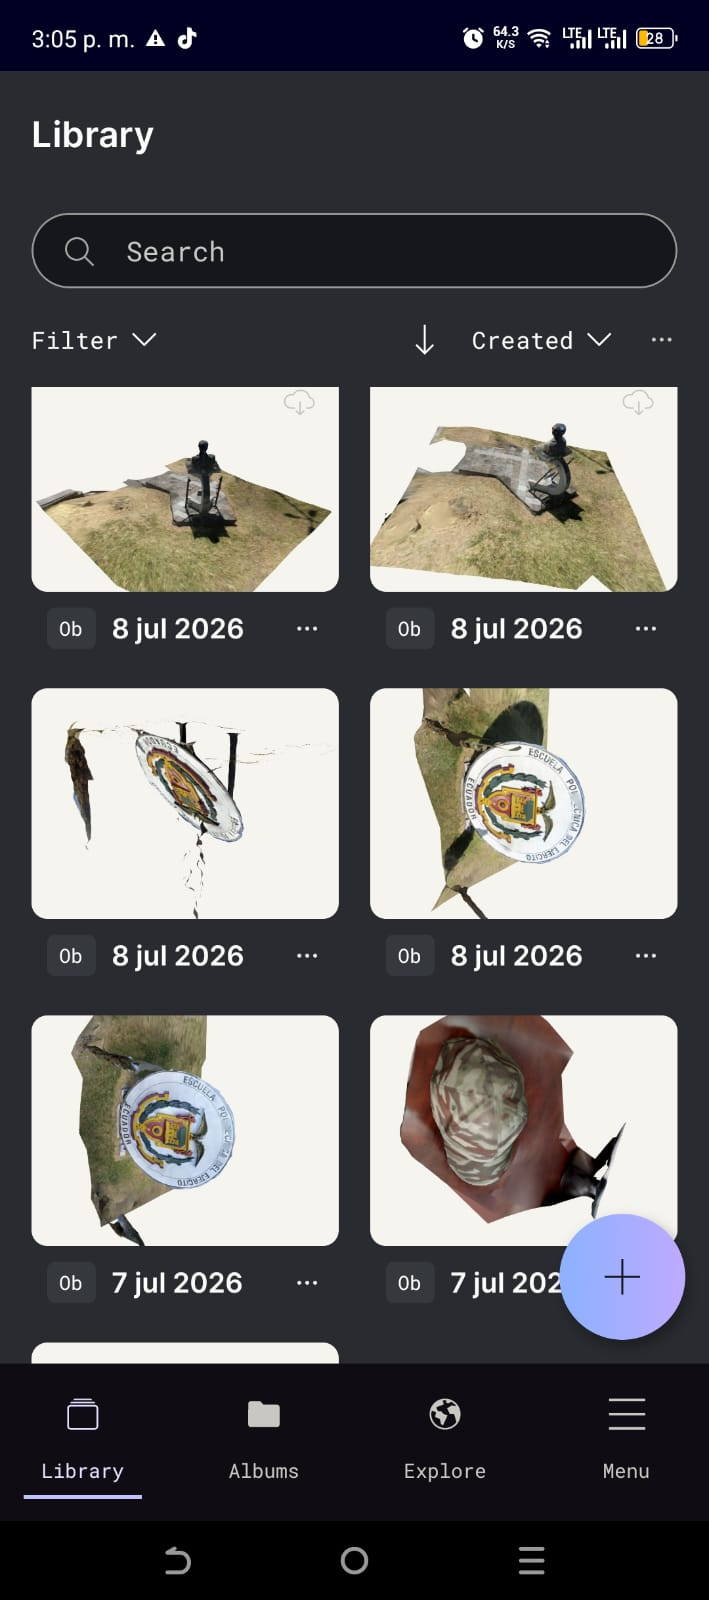
\includegraphics[width=0.45\textwidth]{polycam_captura1.jpg}
    %\includegraphics[width=0.45\textwidth]{polycam_captura2.jpg}
    \caption{Capturas del proceso de escaneo en Polycam.}
\end{figure}

% =================== GENERACIÓN DEL MODELO 3D ===================
\section{Generaci\'on del Modelo 3D}

Una vez obtenido el modelo desde Polycam, se import\'o en \textbf{Blender} para su limpieza y optimizaci\'on. Las tareas realizadas incluyeron:

\begin{itemize}
    \item Eliminaci\'on de geometr\'ia flotante y artefactos generados durante la reconstrucci\'on.
    \item Simplificaci\'on de la malla (decimation) para reducir el n\'umero de pol\'igonos sin perder detalles significativos.
    \item Ajuste de texturas y materiales para mejorar la apariencia visual.
    \item Exportaci\'on final en formato \texttt{.blend} y \texttt{.glb}.
\end{itemize}

\begin{figure}[H]
    \centering
    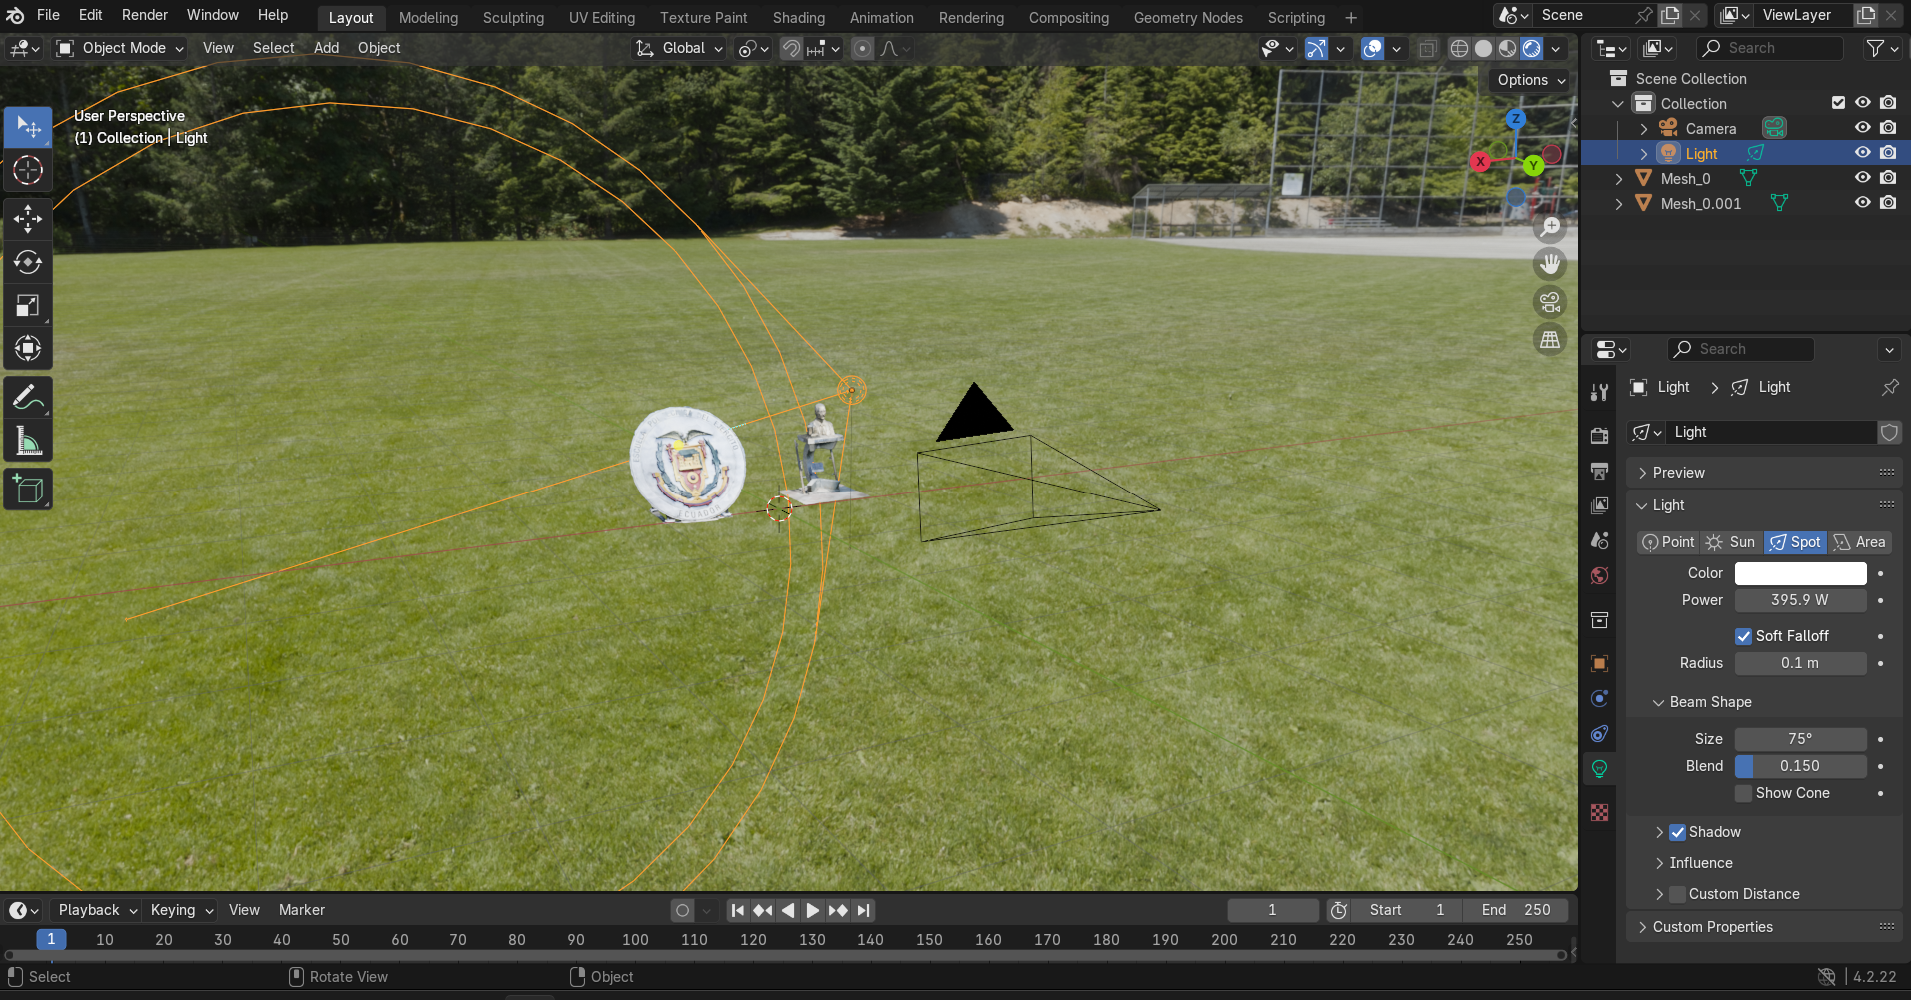
\includegraphics[width=0.8\textwidth]{blender_viewport.png}
    \caption{Modelo 3D del sello en el viewport de Blender.}
\end{figure}

\begin{figure}[H]
    \centering
    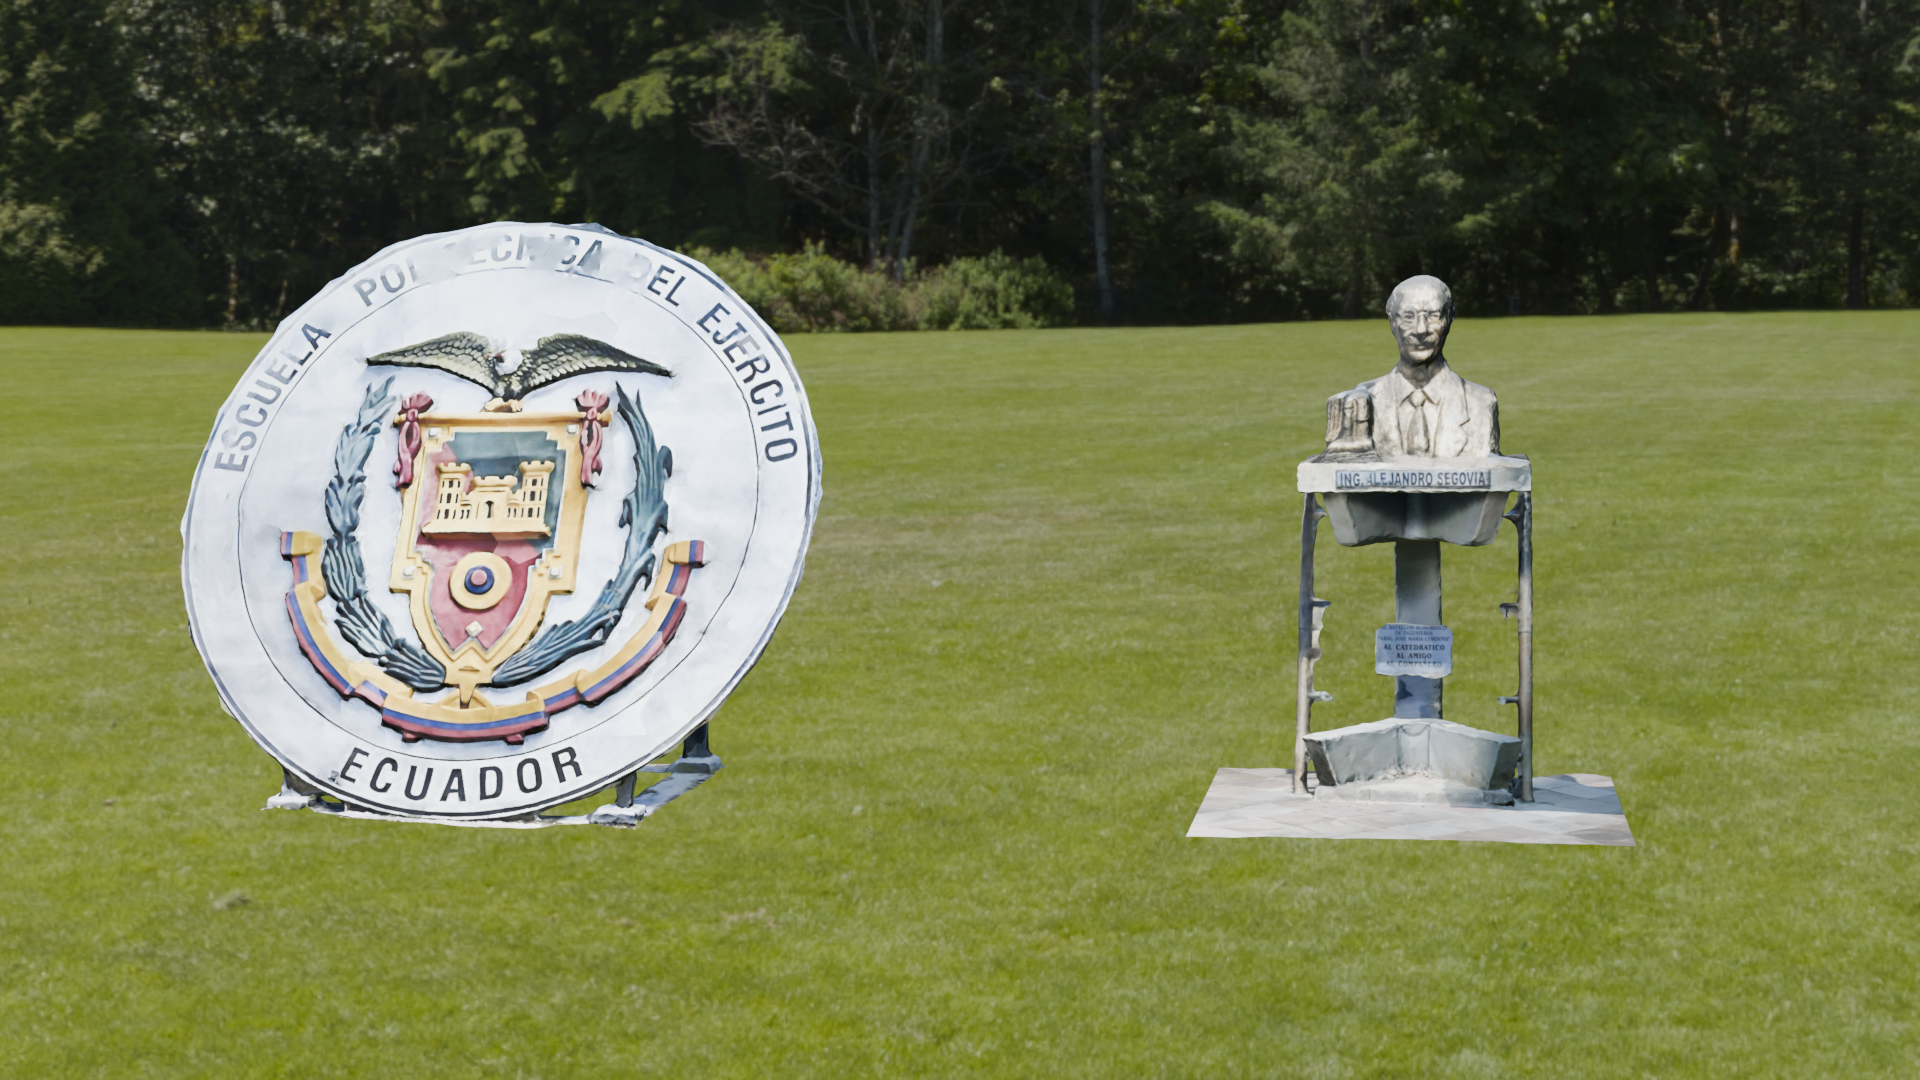
\includegraphics[width=0.8\textwidth]{blender_render.png}
    \caption{Render preliminar del modelo 3D con iluminaci\'on b\'asica.}
\end{figure}

% =================== ANÁLISIS DE RESULTADOS ===================
\section{An\'alisis del Resultado}

\subsection{Calidad del modelo}

El modelo generado presenta una representaci\'on fiel del sello original en cuanto a su forma general y detalles principales. Los elementos en relieve (letras, figuras y bordes) fueron capturados correctamente, aunque se observan algunas \'areas con p\'erdida de definici\'on debido a limitaciones propias de la fotogrametr\'a con dispositivo m\'ovil.

\subsection{Aspectos positivos}

\begin{itemize}
    \item La geometr\'ia general del sello se reconstruy\'o de manera precisa.
    \item Los detalles de mayor tama\~no (como el c\'ondor y las letras principales) son claramente distinguibles.
    \item La textura fotogr\'afica se mape\'o adecuadamente sobre la malla.
    \item El flujo de trabajo Polycam -- Blender result\'o eficiente y accesible.
\end{itemize}

\subsection{Limitaciones observadas}

\begin{itemize}
    \item En \'areas con superficies muy reflectantes o brillantes se perdieron detalles finos.
    \item Algunas zonas con sombras pronunciadas presentaron ruido en la malla.
    \item La resoluci\'on de la c\'amara del dispositivo Android limit\'o la captura de detalles muy peque\~nos.
    \item El modelo requiri\'o limpieza manual en Blender para eliminar artefactos.
\end{itemize}

\subsection{Comparaci\'on con el objeto real}

El modelo 3D obtenido representa fielmente el sello institucional, aunque no alcanza el nivel de detalle de un escaneo profesional con equipo especializado. Para el prop\'osito acad\'emico de la actividad el resultado es satisfactorio, y muestra que la fotogrametr\'a funciona como t\'ecnica de digitalizaci\'on 3D.

\begin{table}[H]
\centering
\caption{Resumen de caracter\'isticas del modelo obtenido.}
\vspace{0.3cm}
\begin{tabular}{|l|l|}
\hline
\textbf{Par\'ametro} & \textbf{Valor} \\ \hline
Herramienta de captura & Polycam (Android) \\ \hline
Formato de exportaci\'on & .glb, .obj, .blend \\ \hline
Software de edici\'on & Blender 4.x \\ \hline
Pol\'igonos aproximados & 150,000 (post-procesado) \\ \hline
Textura & Fotogr\'afica (Polycam) \\ \hline
Tiempo de captura & $\sim$10 minutos \\ \hline
Tiempo de procesamiento & $\sim$5 minutos (nube) \\ \hline
\end{tabular}
\end{table}

% =================== CONCLUSIONES ===================
\section{Conclusiones}

\begin{itemize}
    \item La fotogrametr\'a con Polycam result\'o accesible y efectiva para digitalizar en 3D elementos del campus universitario. El modelo del sello de la ESPE obtenido tiene un nivel de detalle aceptable para fines acad\'emicos.
    \item La iluminaci\'on natural y la captura desde m\'ultiples \'angulos determinaron la calidad del modelo final. Esto confirma que las condiciones de captura deben controlarse en cualquier proceso de fotogrametr\'a.
    \item El posprocesamiento en Blender fue necesario para refinar la malla y corregir artefactos. La fotogrametr\'a autom\'atica, por s\'i sola, no basta: requiere una etapa de edici\'on manual para lograr buenos resultados.
    \item El flujo de trabajo empleado (Polycam $\rightarrow$ Blender $\rightarrow$ archivo .blend/.glb) es un pipeline completo que puede reutilizarse en futuros proyectos acad\'emicos de digitalizaci\'on 3D.
\end{itemize}

\end{document}
